\documentclass[a4paper,14pt]{extarticle}
\usepackage{../../tex-shared/report-layout}

\renewcommand{\mylabnumber}{4}
\renewcommand{\mylabtitle}{Исследование возможнойстей
библиотеки JQuery}
\renewcommand{\mysubject}{Веб-технологии}
\renewcommand{\mylecturer}{Дрозин А.Ю.}

\begin{document}
\begin{titlepage}
    
    \thispagestyle{empty}
    
    \begin{center}
        
        Министерство науки и Высшего образования Российской Федерации \\
        Севастопольский государственный университет \\
        Кафедра ИС
        
        \vfill

        Отчет \\
        по лабораторной работе №\mylabnumber \\
        \enquote{\mylabtitle} \\
        по дисциплине \\
        \enquote{\MakeTextUppercase{\mysubject}}

    \end{center}

    \vspace{1cm}

    \noindent\hspace{7.5cm} Выполнил студент группы ИС/б-17-2-о \\
    \null\hspace{7.5cm} Горбенко К. Н. \\
    \null\hspace{7.5cm} Проверил \\
    \null\hspace{7.5cm} \mylecturer

    \vfill

    \begin{center}
        Севастополь \\
        \the\year{}
    \end{center}

\end{titlepage}

\section{Цель работы}
Изучить возможность программирования на клиентской стороне с
использованием библиотеки jQuery. Приобрести практические навыки использования
библиотеки jQuery для обработки форм, модификации содержимого HTML-страницы,
создания эффектов анимации.

\section{Задание на работу}
\begin{enumerate}
    \item Модифицировать JavaScript, разработанные при выполнении
          предыдущих лабораторных работ, используя везде, где возможно библиотеку
          jQuery для выполнения поставленных задач.
    \item Модифицировать страницу «Фотоальбом», добавив возможность
          просмотра увеличенных версий изображений. При щелчке по стрелкам
          должна происходить анимированная смена изображений.
    \item Реализовать возможность отображения всплывающего блока Popover,
          который показывается рядом с элементом, если на него наводится
          указатель мыши и который исчезает через M секунд после того,
          как указатель мыши покидает элемент.
    \item Использовать разработанный код для отображения подсказок уточняющих
          формат ввода пользователю в формах.
    \item Реализовать возможность отображения всплывающего модального окна,
          которое показывается в центре экрана. При этом задний фон вокруг
          модального окна должен размываться.
\end{enumerate}

\section{Ход работы}
\subsection{Использование JQuery для работы с DOM}
Используем JQuery где возможно для работы с DOM. Выведение истории:
\begin{lstlisting}
const globalHistory = getGlobalHistory();
for (let key in globalHistory) {
    $(`.global-history .${key}-page`).append(globalHistory[key]);
}
const sessionHistory = getSessionHistory();
for (let key in sessionHistory) {
    $(`.session-history .${key}-page`).append(sessionHistory[key]);
}
\end{lstlisting}

В данном случае используются функции \code{append} для вставки контента в элемент \code{td} таблицы.

Валидация форм:
\begin{lstlisting}
const validateForm = (event, fields) => {
    let firstError : FormComponent;
    fields.forEach(field => {
        validateField(field);
        if (!firstError && field.errorMessages.length > 0) {
            firstError = field;
        }
    });
    if (firstError) {
        $(`#${firstError.componentId}`).trigger('focus');
    }
    if (fields.some(field => field.errorMessages.length > 0)) {
        event.preventDefault();
    }
};

const validateField = (field: FormComponent) => {
    const presentErrorMessages = $(`#${field.componentId}-errors`);
    if (presentErrorMessages.length > 0) {
        presentErrorMessages.remove();
        $(`#${field.componentId}`).removeClass('validation-failed');
    }
    field.validate();
    if (field.errorMessages.length > 0) {
        showMessages(field);
    }
};

const showMessages = (field: FormComponent) => {
    const targetElement = $(`#${field.componentId}`).addClass('validation-failed');
    let contentWrapper = $('<div></div>').attr('id', `${field.componentId}-errors`).addClass('error-messages');
    field.errorMessages.forEach(message => contentWrapper.append($(`<li>${message}</li>`)));
    contentWrapper.insertBefore(targetElement);
};
\end{lstlisting}

JQuery использовался для всевозможный манипуляций DOM:  отображения/сокрытия элементов,
выборки объектов из DOM, добавления и удаления классов и атрибутов.

\subsection{Реализация просмотра фотографий}
Реализуем просмотр фотографий:

\begin{lstlisting}
import * as $ from 'jquery';

let body = $('body');
let lightbox = $('#lightbox');
let lightboxImage = $('#lightbox img');
let lightboxPrevArrow = $('.lightbox-arrow-left');
let lightboxNextArrow = $('.lightbox-arrow-right');

let currentPhoto;
let photos;

export default (lightboxPhotosWrapper: Element, photosPaths: string[]) => {
    photos = photosPaths;
    lightboxPhotosWrapper.addEventListener('click', (event) => expandLightbox(event));

    window.onclick = (event) => {
        if (event.target === document.getElementById('lightbox')) {
            collapseLightbox();
        }
    }
}

const expandLightbox = (event) => {
    currentPhoto = event.target.getAttribute('src');
    lightbox.toggle();
    lightboxImage.attr('src', currentPhoto);
    body.addClass('no-scroll');
    lightboxPrevArrow.on('click', prevButtonClickHandler);
    lightboxNextArrow.on('click', nextButtonClickHandler);
};

const collapseLightbox = () => {
    lightbox.toggle();
    body.removeClass('no-scroll');
};

const prevButtonClickHandler = () => {
    const currentIndex = photos.indexOf(currentPhoto);
    if (currentIndex === 0 || currentIndex === -1) return;
    currentPhoto = photos[currentIndex - 1];
    lightboxImage.attr('src', currentPhoto);
};

const nextButtonClickHandler = () => {
    const currentIndex = photos.indexOf(currentPhoto);
    if (currentIndex === photos.length - 1 || currentIndex === -1) return;
    currentPhoto = photos[currentIndex + 1];
    lightboxImage.attr('src', currentPhoto);
};
\end{lstlisting}

В данном файле реализуется включение отображения окна просмотра фотографий. На кнопки назад/далее
навешиваются обработчики событий с проверкой выхода за границы массива.

Получившийся элемент имеет следующий вид (рисунок \ref{fig:photos}):
\begin{figure}[H]
    \centering
    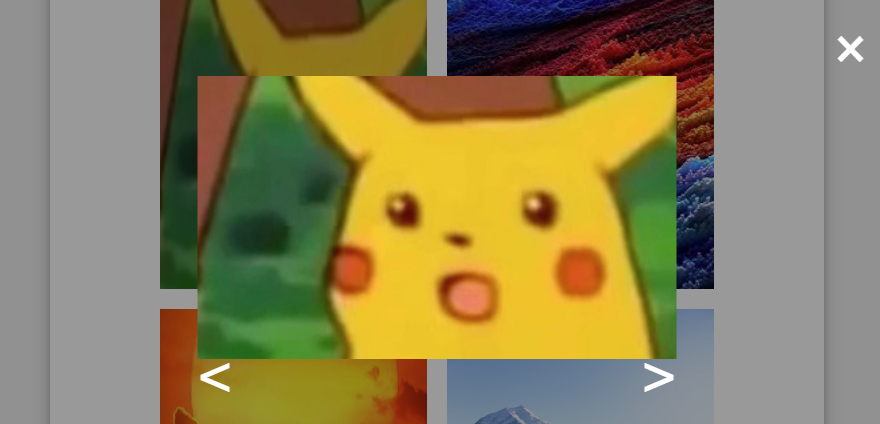
\includegraphics[width=.8\linewidth]{photos}
    \caption{Вид реализации переключения фотографий}
    \label{fig:photos}
\end{figure}

\subsection{Реализация всплывающего окна}
Для реализации всплывающего окна была использована сторонняя библиотека
\code{tooltipster}. Ее использование:

\begin{lstlisting}
import 'tooltipster';

export const setFieldsForValidation = (fields: FormComponent[], form: HTMLFormElement) => {
    $(form).on('submit', (event) => validateForm(event, fields));
    fields.forEach(formComponent => {
        const field =  $(`#${formComponent.componentId}`);
        field.on('blur', () => validateField(formComponent));
        field.tooltipster({ content: formComponent.correctValueDescription, theme: 'tooltipster-light', side: 'right' });
    });
};
\end{lstlisting}

Реализованный компонент имеет следующий вид (рисунок \ref{fig:popover}):
\begin{figure}[H]
    \centering
    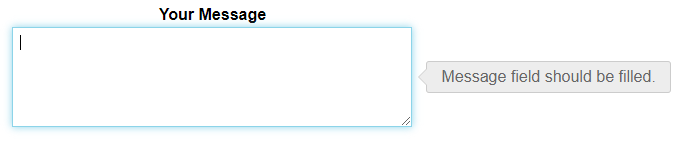
\includegraphics[width=.8\linewidth]{popover}
    \caption{Вид реализации всплювающего окна}
    \label{fig:popover}
\end{figure}

\section{Реализация модального окна}
Реализуем модальное окно:

\begin{lstlisting}
import * as $ from 'jquery';

export interface IModalOptions {
    message?: string;
    confirmButtonText?: string;
    cancelButtonText?: string;
    confirmAction?: () => void;
    cancelAction?: () => void;
}

const body = $('body');
const getModal = () => $('.modal');
const message = 'Do you really want to do this?';
const confirmButtonText = 'Yes';
const cancelButtonText = 'No';

export default (options: IModalOptions) => {
    $('.modal-message').text(options.message || message);
    $('.modal-confirm-button').text(options.confirmButtonText || confirmButtonText).off('click').on('click', getAction(options.confirmAction));
    $('.modal-cancel-button').text(options.cancelButtonText || cancelButtonText).off('click').on('click', getAction(options.cancelAction));
    expandModal();
}

const expandModal = () => {
    body.addClass('no-scroll');
    getModal().toggle();
};

const collapseModal = () => {
    body.removeClass('no-scroll');
    getModal().toggle();
};

const getAction = (action: () => void) => {
    if (action) {
        return () => { collapseModal(); action(); }
    }
    return () => collapseModal();
};
\end{lstlisting}

Интерфейс модуля модального окна включает объект с настройками: \code{callback}-функции,
вызываемые при нажатии на подтверждение или отмену, тексты кнопок, сообщение.

Элемент имеет следующий вид (рисунок \ref{fig:modal}):
\begin{figure}[H]
    \centering
    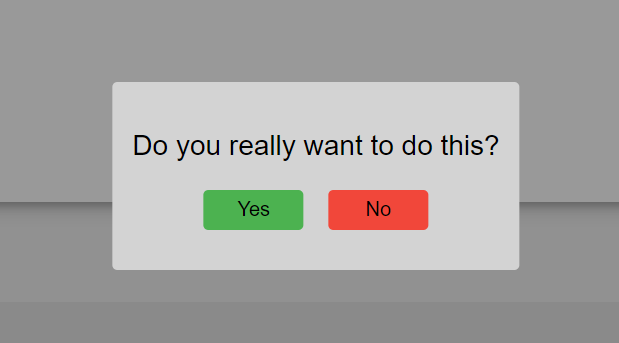
\includegraphics[width=.8\linewidth]{modal}
    \caption{Вид реализации модального окна}
    \label{fig:modal}
\end{figure}

\section*{Выводы}
В ходе лабораторной работы была исследована библиотека JQuery. Лна была использована
для упрощения работы с DOM.

Преимущества JQuery следующие: упрощенная работа с выборкой элементов из DOM,
богатая библиотека для работы с обектами JQuery, легко трансформируемыми в объекты DOM,
возможность последовательного вызова функций.
\end{document}